\section{Lezione 13}

UML mette a disposizione gli \textbf{eventi esterni}, l'invio e la ricezione di messaggi a un altro diagramma di attività (quindi verso l'esterno). Quando voglio ricevere un messaggio dall'utente l'elaborazione viene bloccata in attesa della ricezione. Queste due primitive individuano il concetto di \textbf{sincronizzazione}.

La \textit{clessidra} è un \textbf{timer}, verifica il passaggio del tempo.

\begin{center}
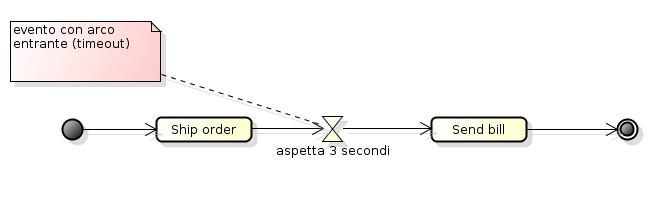
\includegraphics[width=0.75\columnwidth]{img1} % Example image
\end{center}

Gli archi che connettono due azioni servono per generare un flusso da un'azione a un'altra. È possibile spezzare un arco in due con una notazione sotto forma di etichetta. Possiamo anche volendo passare un oggetto da un'azione a un'altra.

\begin{center}
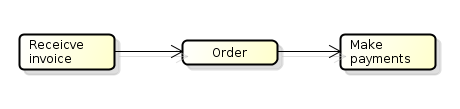
\includegraphics[width=0.75\columnwidth]{img2} % Example image
\end{center}

Le \textbf{regioni di esposizione} sono utili quando bisogna fare delle azioni su delle collezioni. Ogni elemento della lista è un \textit{token}, un solo token in uscita dalla regione.

\begin{center}
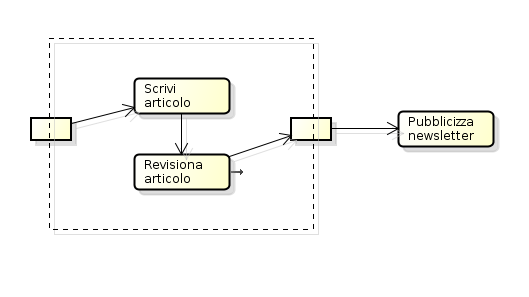
\includegraphics[width=0.75\columnwidth]{img3} % Example image
\end{center}

Non tutti i flussi possono arrivare alla fine, in tal caso può esserci un \textbf{nodo di terminazione} che fa morire un token. I diagrammi di attività sono i diagrammi più utili di tutti. Da utilizzare:

\begin{itemize}

	\item Espressione di flussi paralleli;
	\item Per descrivere casi d'uso o requisiti direttamente dal capitolato tecnico.

\end{itemize}

\textbf{Diagrammi di sequenza}

Capire come due attori interagiscono tra di loro, interazione dinamica nel tempo di due parti. Si usano nella parte di definizione architetturale. Permette a chi dovrà andare a programmare di capire l'architettura e come far collaborare più gruppi di oggetti.

\begin{center}
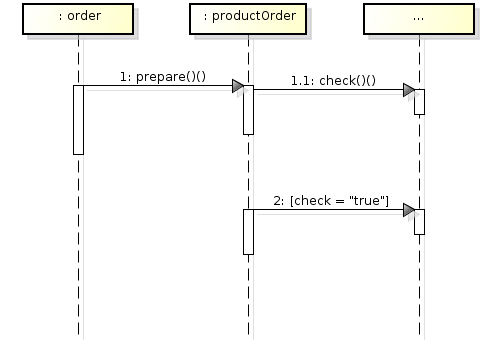
\includegraphics[width=0.75\columnwidth]{img4} % Example image
\end{center}

\begin{center}
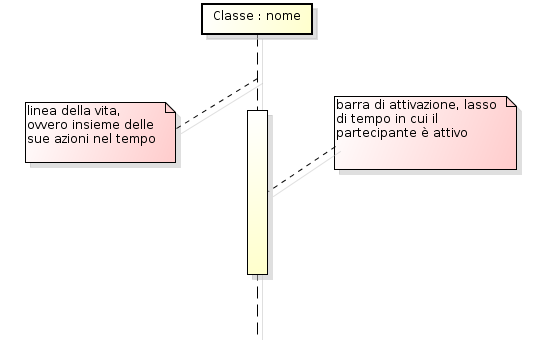
\includegraphics[width=0.75\columnwidth]{img6} % Example image
\end{center}

È interessante vedere come avvengono le interazioni tra più partecipanti. Queste avvengono tramite \textbf{messaggi}. L'inizio di un messaggio si rappresenta con una freccia continua da un partecipante all'altro. È possibile avere anche un messaggio che arriva dall'\textbf{esterno} del partecipante. L'evento esterno attiva il diagramma di sequenza e lo fa partire. Il ritorno di un messaggio è rappresentato da una freccia tratteggiata.

Esistono due possibili messaggi: \textbf{sincroni} e \textbf{asincroni}.

\begin{center}
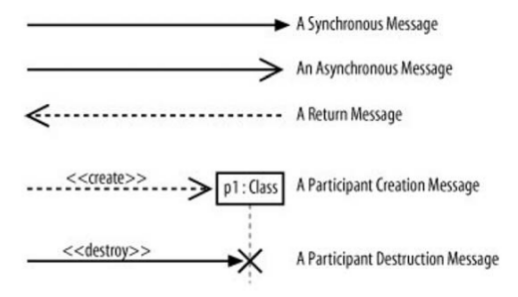
\includegraphics[width=0.75\columnwidth]{img5} % Example image
\end{center}

Un partecipante può creare un altro partecipante (normalmente tramite la \textit{new}), per questo si usa la \textbf{create}:

\begin{center}
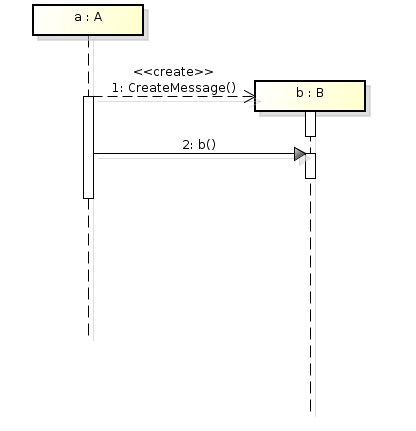
\includegraphics[width=0.75\columnwidth]{img7} % Example image
\end{center}

Di contro un oggetto può richiedere la distruzione di un altro oggetto. In questo caso si invia un altro messaggio e si mette una $X$ sulla linea della vita del partecipante. Un oggetto può anche suicidarsi, ovvero distruggere se stesso.

In UML2 hanno introdotto le primitive per rappresentare i \textbf{cicli} e le \textbf{condizioni} tramite i \textit{frame} di intestazione, ciascuno con un'etichetta che rappresenta qualcosa.

\begin{center}
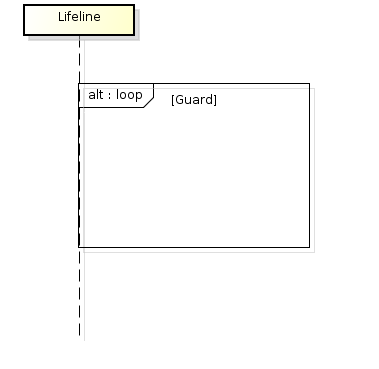
\includegraphics[width=0.75\columnwidth]{img8} % Example image
\end{center}

Ci sono vari \textbf{operatori} (etichette):

\begin{itemize}

	\item \textbf{ALT};
	\item \textbf{OPT};
	\item \textbf{PAR};
	\item \textbf{LOOP};
	\item \textbf{REGION};
	\item \textbf{NEG};
	\item \textbf{REF};
	\item \textbf{SD}.

\end{itemize}

Se ho bisogno di modellare la collaborazione uso i diagrammi di sequenza, se devo modellare algoritmi uso i diagrammi di attività.

Controllo \textbf{centralizzato} e \textbf{distribuito}. Bisogna cercare di delegare il più possibile agli oggetti le operazioni su se stessi (\textit{delegation pattern}). Nel contratto distribuito non abbiamo più un registro che \textit{schedula} tutte le attività, ma tutto parte da un singolo oggetto che invoca metodi su altri oggetti, manda e riceve messaggi.

\textbf{Esercizio}:

\begin{center}
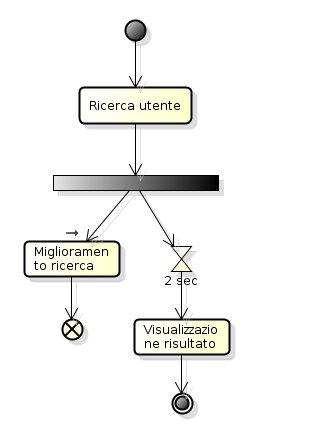
\includegraphics[width=0.75\columnwidth]{img9} % Example image
\end{center}